%!TEX program = xelatex

% 纸张模式:护眼模式-geye 朦胧模式-hazy
% 纸张尺寸:pad kindle pc normal screen
\documentclass[cn, blue, normal, 12pt]{elegantnote}

\title{软件工程复习笔记}
\author{Xiaohei}
\institute{Created by Elegant\LaTeX{}}
\version{0.1}
\date{\zhtoday}

\begin{document}

\maketitle

\section{软件工程学概述}

复习内容:

\begin{enumerate}
    \item 了解软件工程的诞生及软件的特点
    \item 了解软件危机
    \item 掌握软件工程的三个基本要素
    \item 了解软件生命周期的含义及各阶段的任务
    \item 了解软件过程各模型的适用范围
\end{enumerate}

\subsection{软件工程学}

迄今为止,人们仍然没有彻底摆脱“\textbf{软件危机}”的困扰,软件已经成为限制计算机系统发展的瓶颈。软件工程概念的提出是为了解决\textbf{软件危机}。

软件工程的诞生:1968年北大西洋公约组织召开国际会议,提出“软件工程”概念和术语。

软件工程的目标:创造“\textbf{足够好}”的软件。

\subsection{软件的特点}

软件包括:为实现设计的功能和性能要求的\textbf{指令集};使程序能正常运行的\textbf{数据};与程序开发、维护和使用有关的\textbf{文档}。

\subsection{软件危机}

软件危机就是指在软件开发和软件维护过程中所存在的一系列\textbf{严重问题}。

产生软件危机的原因:软件具有\textbf{复杂性}、\textbf{演化性}、\textbf{服从性}、\textbf{不可见性}。

\subsection{软件生命周期}

软件生命周期指一个软件\textbf{从提出开发要求开始直到不再使用(报废)为止}的整个时期。

软件生存周期阶段划分为三个时期:\textbf{软件定义、软件开发、软件使用和维护}。

软件定义时期:问题定义、可行性研究、需求分析。

软件开发时期:概要设计、详细设计、编码及单元测试、综合测试。

软件维护时期:改正性维护、适应性维护、完善性维护、预防性维护。

\subsection{软件工程方法学}

软件工程方法学的三要素:\textbf{过程、方法、工具}。

\subsection{软件过程}

\textbf{软件过程}描述为了开发出客户需要的软件,什么人、在什么时候、做什么事以及怎样做这些事以实现某一个特定的具体目标。

\textbf{软件过程模型}定义软件开发过程中所需要完成的活动、活动之间的顺序以及活动之间的关系。

\subsubsection{瀑布模型}

瀑布模型也称经典生命周期模型,开发阶段严格按照线性方式进行
,每一个阶段具有相关的里程碑和交付产品,且需要确认和验证。

瀑布模型适用于\textbf{系统需求明确且稳定、技术成熟、工程管理较严格}的场合。如军工、航天、医疗。

\subsubsection{快速原型模型}

快速原型是快速构建一个可运行的软件原型,用户和开发人员通过对原型的检查来决定原型是否合适和恰当。

快速原型模型适用于\textbf{客户不清楚系统的具体输入输出,开发者不确定算法效率、计算机交互的方式}等场合。

\subsubsection{增量模型}

把软件产品作为一系列的增量构件来设计、编码、集成和测试。每
个构件由多个相互作用的模块构成,并且能够完成特定的功能。

增量模型适用于\textbf{软件开发中需求可能发生变化、具有较大风险、或者希望尽早进入市场}的项目。

\subsubsection{Rational统一过程模型}

由Rational公司推出的完整的软件工程方法,已获得广泛使用。基于面向对象方法学,使用统一建模语言UML(Unified Modeling Language),适合\textbf{大团队、大项目}。

\subsubsection{敏捷开发过程}

敏捷开发是一种基于更紧密的团队协作、能够有效应对快速变化需求、快速交付高质量软件的迭代和增量的新型软件开发方法。

敏捷开发过程适用于\textbf{需求模糊且经常改变的场合},适合\textbf{商业竞争环境下的项目}。

最有影响的两个敏捷开发方法是Scrum开发方法和极限编程(XP)。

\section{需求分析}

复习内容:

\begin{enumerate}
    \item 了解面向过程和面向对象分析模型有哪些描述工具
    \item 掌握数据流图
    \item 掌握数据字典的定义、作用和组成条目
    \item 掌握用例图
    \item 了解类图的组成和类与类之间的关系
    \item 了解其他需求分析阶段的图形工具
    \item 掌握验证软件需求的正确性的四个方面
\end{enumerate}

\subsection{分析模型的描述工具}

\begin{table}[htbp]
    \centering
    \begin{tabular}{c|c|c}
    \toprule
            & 面向过程的需求分析 & 面向对象的需求分析   \\
    \midrule
    数据模型 & 实体-联系图、数据字典 & 类图、类关系图   \\
    功能模型 & 数据流图(DFD)    & 用例图             \\
    行为模型 & 状态变迁图(STD) & 活动图、时序图、状态图 \\
    \bottomrule
    \end{tabular}
\end{table}

\subsection{数据流图}

数据流图是从数据传递和加工的角度,以图形的方式刻画数据流从输入到输出的移动变换过程。

\textbf{数据流}是数据在系统中的传送通道,数据流符号的箭头指明了数据的流动方向,由一组固定成分的数据组成。数据流可从加工流向加工,也可在加工与数据存储或外部项之间流动;两个加工之间可有多股数据流。

\textbf{加工}表示对数据进行的操作,如“处理选课单” 等。每个加工至少有一个输入数据流和一个输出数据流。加工的编号是这个加工在层次分解中的位置。

\textbf{数据存储}是用于保存数据的数据文件,它可以是数据库文件或
任何其他形式的数据组织。

\textbf{外部实体}(数据源点/终点)是反映数据流图与外部实体之间的联系,表示图中的输入数据来自哪里或处理结果送向何处。

\begin{figure}[htbp]
    \centering
    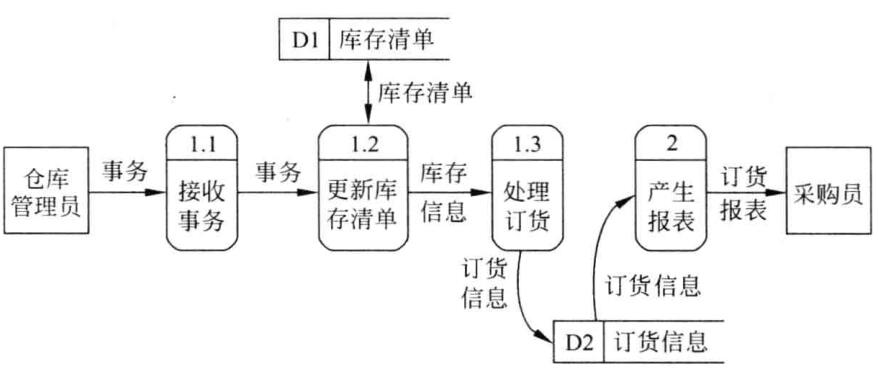
\includegraphics[width=0.8\textwidth]{数据流图.jpg}
\end{figure}

\subsection{数据字典}

\textbf{数据字典}是数据流图的补充,能够准确地定义数据流图中各组成成分的具体含义。

数据字典用简洁、清晰、易理解的文字描述条目,说明数据流图的加工功能、性能、要求及设计约束等。

数据流图和数据字典共同构成了系统的功能逻辑模型。

数据字典的组成:\textbf{数据流条目、数据项条目、数据文件条目、数据加工条目}。

\subsection{用例图}

用例建模用于描述系统需求,把系统当作黑盒,从用户的角度,描述系统的场景。主要的图形元素有:参与者、用例。

\textbf{参与者}:是指外部用户或外部实体在系统中扮演的角色。 可以是一个人、一个硬件设备等。

\textbf{用例}:对一组动作序列的描述,系统通过执行这一组动作序列为参与者产生一个可观察的结果。用例名往往用动宾结构命名。

\textbf{系统}:用于界定系统功能范围,描述该系统功能的用例都置于其中,而描述外部实体的参与者都置于其外。

用例图中的四种关系:\textbf{关联、泛化、包含、扩展}。

\textbf{关联}:参与者与用例之间的通信,任何一方都可发送或接受消息。箭头指向消息接收方。

\textbf{泛化}:就是通常理解的继承关系,子用例和父用例相似,但表现出更
特别的行为;子用例可以重载父用例。父用例通常是抽象的。箭头由子用例指向父用例,箭头为空箭头。

\textbf{包含}:当多个用例有共享行为时,应该使用包含的关系来表示它们。箭头由基本用例指向共享用例,连线为虚线。

\textbf{扩展}:扩展关系是指用例功能的延伸,相当于为基础用例提供一个附加功能。 由一个用例的扩展点可以扩展出另外一个用例。箭头指向基础用例,连线为虚线。

包含关系中,在执行基本用例时,一定会执行包含用例部分;扩展关系中,一个基本用例执行时,可以执行或不执行扩展用例部分。

\begin{figure}[htbp]
    \centering
    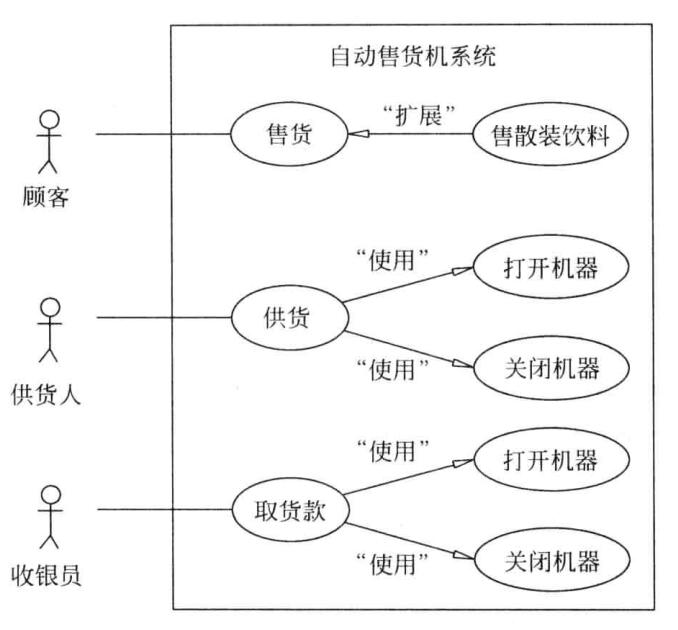
\includegraphics[width=0.5\textwidth]{用例图.jpg}
\end{figure}

\subsection{类图}

类图是由若干类关联在一起,反映系统或者子系统组成结构的静态图。

类图的组成:\textbf{类、关联}。

\textbf{类}:是具有共同结构特征、行为特征、联系和语义的对象集合的抽象形式。

\textbf{关联}:表示类与类之间的关系。

类在UML中通常以实线矩形框表示,矩形框中含有若干分隔框,分别包含类的名字、属性、操作、约束以及其他成分等。

类的属性在UML类图标的矩形框中用文字串说明。“:”后跟属性值的数据类型,可通过在属性名和数据类型后添加“=”为属性指定初始值。

操作(方法)是类提供的功能服务,在类矩形框中用文字串说明。

类的关系:\textbf{关联关系(聚合、组合)、依赖关系、泛化关系}等。

\textbf{关联关系}:\textbf{聚合}描述整体和部分的关系,其中一个类为整体,它由一个或多个部分类组成。在聚合中,部分类可以没有整体类而存在。聚合使用\textbf{带有空心菱形的实线}连接。\textbf{组合}是特殊的聚合关联。组合关联中组成整体类的部分类不能独立存在,需要整体类才能存在。组合使用\textbf{带有实心菱形的实线}连接。

\textbf{依赖关系}:指一个类的元素使用了另一个类。依赖关系描述类之间的引用关系。使用带箭头的虚线连接。

\textbf{泛化关系}:描述类之间的继承关系。利用泛化来表达类之间的相似性,子类共享父类的属性和操作。使用带空心箭头的实线连接。

\begin{figure}[htbp]
    \centering
    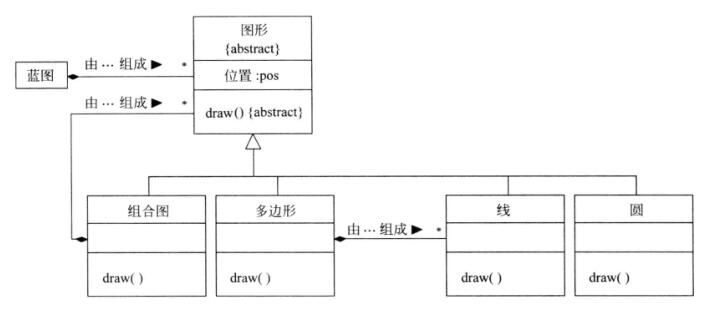
\includegraphics[width=0.8\textwidth]{类图.jpg}
\end{figure}

\subsection{其他图形工具}

\textbf{状态转换图}:通过描绘系统的状态及引起系统状态转换的事件,来表示系统的行为。状态图还指明了作为特定事件的结果系统将做哪些动作。

\begin{figure}[htbp]
    \centering
    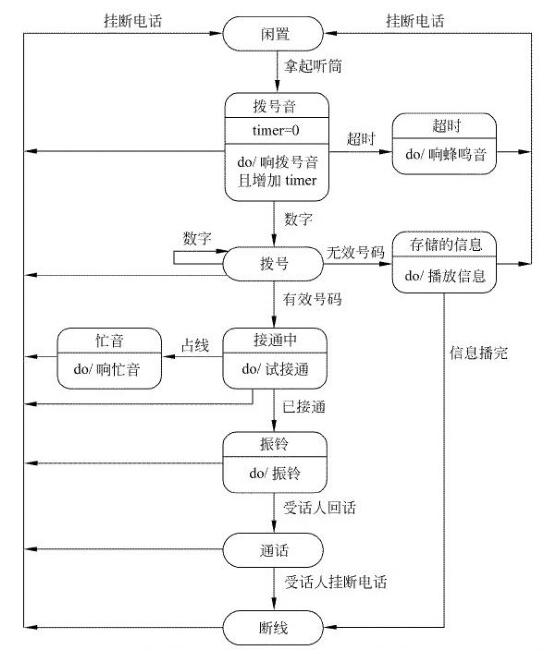
\includegraphics[width=0.68\textwidth]{状态转换图.jpg}
\end{figure}

\textbf{层次方框图}:用树形结构的一系列多层次的矩形框描述复杂数据的层次结构。从对顶层信息的分类开始,沿着层次图中的每条路径逐步细化,直到确定了数据结构的全部细节为止。

\begin{figure}[htbp]
    \centering
    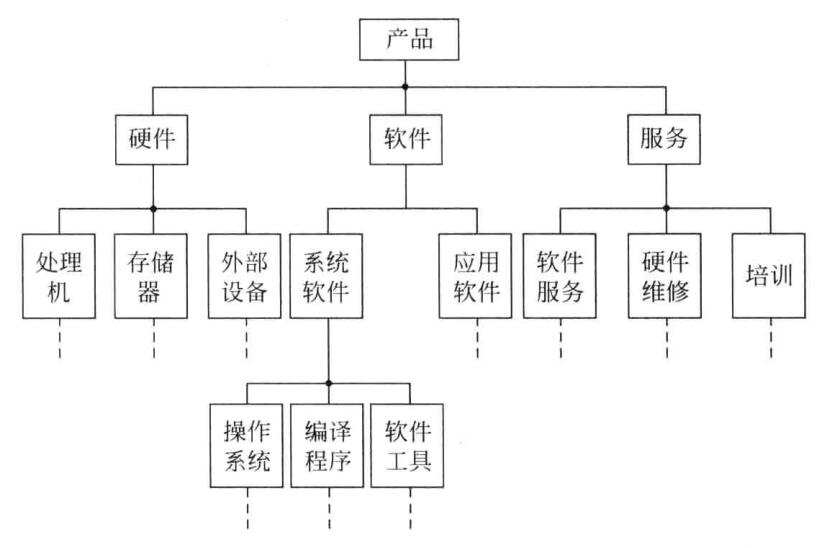
\includegraphics[width=0.65\textwidth]{层次方框图.jpg}
\end{figure}

\textbf{Warnier图}:与层次方框图类似,但提供了更丰富的描绘手段,可更清楚地描述信息的逻辑组织。

\begin{figure}[htbp]
    \centering
    \includegraphics[width=0.65\textwidth]{Warnier图.jpg}
\end{figure}

\subsection{验证软件需求}

\textbf{验证需求的一致性}:所有需求必须是一致的,任何一条需求不能和其他需求互相矛盾。

\textbf{验证需求的完整性}:需求必须是完整的,需求规格说明书中应包括用户需求的每一个功能或性能。

\textbf{验证需求的有效性}:必须证明需求是正确有效的,确实能够解决用户面对的问题。

\textbf{验证需求的现实性}:需求在现有硬件和软件技术水平上应该是能够实现的。

\section{总体设计}

复习内容:

\begin{enumerate}
    \item 掌握总体设计的设计原理
    \item 掌握软件结构设计的启发式规则
    \item 了解顺序图的作用及组成
\end{enumerate}

\subsection{总体设计过程}

总体设计的基本目的就是回答“概括地说,系统应该如何实现”这个问题,因此,总体设计又称为概要设计或初步设计。

总体设计的设计原理:\textbf{模块化、抽象、逐步求精、信息隐藏、模块独立}。

\textbf{模块化}:模块化的依据是使问题复杂度降低,易实现易理解。模块数目增加时每个模块的规模将减小,开发单个模块的工作量也将减少。但同时增加了设计模块接口的工作量。

\textbf{抽象}:将现实世界中具有共性的一类事物的相似的、本质的方面集中概括起来,而暂时忽略它们之间的细节差异。

\textbf{逐步求精}:为了能集中精力解决主要问题而尽量推迟对问题细节的考虑。逐步求精最初是自顶向下的设计策略,程序的体系结构通过逐步精化处理过程的层次设计出来。

\textbf{信息隐藏}:模块内部的信息对于不需要这些信息的模块来说是不能访问的。提高模块的独立性,模块之间的信息传递只能通过\textbf{合法的调用接口}来实现。

\textbf{模块独立}:模块独立的概念是模块化、抽象、信息隐蔽概念的直接结果。模块独立程度的度量标准:\textbf{耦合}:衡量\textbf{不同模块之间}相互依赖程度的度量指标;\textbf{内聚}:衡量\textbf{一个模块内部各元素}相互依赖程度的度量指标。

\textbf{耦合}

\begin{enumerate}
    \item \textbf{数据耦合}:如果两个模块彼此间通过参数交换信息,交换的信息只有数据。
    \item \textbf{控制耦合}:模块之间交换的信息中包含有控制信息。
    \item \textbf{特征耦合}:把整个数据结构作为参数传递而被调用的模块只需要使用其中一部分数据元素。
    \item \textbf{公共耦合}:两个或多个模块通过引用公共数据相互联系。
    \item \textbf{内容耦合}:一个模块访问另一模块的内部数据;一个模块不通过正常入口而转到另一模块内部;两个模块有一部分程序代码重叠;一个模块具有多个入口。
\end{enumerate}

数据耦合是低耦合,内容耦合是所有耦合关系中程度最高的。

\textbf{内聚}

\begin{enumerate}
    \item \textbf{偶然内聚}:一个模块完成一组任务,这些任务彼此间即使有关系,关系也是很松散的。
    \item \textbf{逻辑内聚}:一个模块完成的任务在逻辑上属相同或相似的一类。
    \item \textbf{时间内聚}:一个模块包含的任务必须在同一段时间内执行。
    \item \textbf{过程内聚}:一个模块内的处理元素是相关的,而且必须以特定次序执行。
    \item \textbf{通信内聚}:模块中所有元素都使用同一个输入数据和(或)产生同一个输出数据。
    \item \textbf{顺序内聚}:一个模块内的处理元素和同一个功能密切相关,而且这些处理必须顺序执行,通常前一部分的输出作为后一部分的输入。
    \item \textbf{功能内聚}:模块内所有处理元素属于一个整体,完成一个单一的功能。
\end{enumerate}

功能内聚是最高程度的内聚。

\subsection{启发式规则}

\textbf{改进软件结构提高模块独立性}:通过模块分解或合并,\textbf{降低耦合提高内聚}。

\textbf{模块规模应该适中}:一个模块的规模不应过大,通常不超过60行语句。

\textbf{深度、宽度、扇出和扇入都应适当}:顶层高扇出,中层低扇出,底层高扇入。

深度:软件结构中控制的层数,粗略地标示一个系统
的大小和复杂程度。

宽度:软件结构内同一个层次上模块总数的最大值,
一般来说,宽度越大的系统越复杂。

扇入:一个模块被多少个上级模块直接调用的数目。

扇出:一个模块直接控制(调用)的下级模块数目。

\textbf{模块的作用域应该在控制域范围之内}

作用域:受该模块内一个判定影响的所有模块范围。

控制域:模块本身及所有直接或间接从属于它的模块。

\textbf{力争降低模块接口的复杂程度}:模块接口设计原则是易理解,传递信息简单且与模块功能一致。

\textbf{设计单入口单出口的模块}:不要使模块间出现内容耦合。当从顶部进入模块并且从底部退出来时,软件是比较容易理解的,因此也是比较容易维护的。

\textbf{模块功能应该可以预测}:相同的输入应产生相同的输出。

\subsection{顺序图}



\section{详细设计}

复习内容:

\begin{enumerate}
    \item 了解结构程序设计的要求
    \item 掌握详细设计工具(程序流程图、盒图、PAD图)
\end{enumerate}

\section{实现}

复习内容:

\begin{enumerate}
    \item 了解编码风格,测试的目的
    \item 了解白盒测试的概念,掌握不同覆盖标准测试用例的选择(语句、条件、路径)
    \item 了解黑盒测试的概念,了解三种黑盒测试方法
    \item 了解单元测试、集成测试、确认测试的目标和方法
\end{enumerate}

\end{document}
